% ============================================================
% 35-bezier-interactive-explained.tex
% Compile with:  pdflatex -shell-escape 35-bezier-interactive-explained.tex
% All three PNGs must be in the same folder. Run twice for TOC.
% ============================================================

\documentclass[12pt, a4paper]{article}

\usepackage[T1]{fontenc}
\usepackage[utf8]{inputenc}
\usepackage{lmodern}
\usepackage[top=2.5cm, bottom=2.5cm, left=2.8cm, right=2.8cm]{geometry}
\usepackage{graphicx}
\usepackage{float}
\usepackage[dvipsnames]{xcolor}

\definecolor{codebg}{RGB}{248,248,248}
\definecolor{rulecolor}{RGB}{180,180,180}
\definecolor{examplebg}{RGB}{240,248,255}
\definecolor{examplerule}{RGB}{100,149,237}
\definecolor{notebg}{RGB}{255,250,230}
\definecolor{noterule}{RGB}{210,180,50}
\definecolor{samebg}{RGB}{245,245,245}
\definecolor{samerule}{RGB}{160,160,160}

\usepackage{minted}
\setminted[julia]{
  bgcolor=codebg, frame=leftline, framerule=1.5pt,
  rulecolor=rulecolor, linenos=false, fontsize=\small,
  breaklines=true, tabsize=4, style=friendly,
}

\usepackage{amsmath}
\usepackage{amssymb}
\usepackage{tikz}
\usetikzlibrary{shapes.geometric, arrows.meta, positioning, fit}
\usepackage{mdframed}

\newmdenv[backgroundcolor=examplebg, linecolor=examplerule,
  linewidth=1.5pt, leftline=true, rightline=false,
  topline=false, bottomline=false,
  innerleftmargin=10pt, innerrightmargin=8pt,
  innertopmargin=6pt, innerbottommargin=6pt,
  skipabove=6pt, skipbelow=4pt]{examplebox}

\newmdenv[backgroundcolor=notebg, linecolor=noterule,
  linewidth=1.5pt, leftline=true, rightline=false,
  topline=false, bottomline=false,
  innerleftmargin=10pt, innerrightmargin=8pt,
  innertopmargin=6pt, innerbottommargin=6pt,
  skipabove=6pt, skipbelow=4pt]{notebox}

\newmdenv[backgroundcolor=samebg, linecolor=samerule,
  linewidth=1.5pt, leftline=true, rightline=false,
  topline=false, bottomline=false,
  innerleftmargin=10pt, innerrightmargin=8pt,
  innertopmargin=6pt, innerbottommargin=6pt,
  skipabove=6pt, skipbelow=4pt]{samebox}

\usepackage[colorlinks=true, linkcolor=black, urlcolor=MidnightBlue]{hyperref}
\usepackage{booktabs}
\usepackage{needspace}
\usepackage{parskip}
\usepackage{titlesec}
\usepackage{fancyhdr}
\usepackage{datetime2}

\titleformat{\section}
  {\large\bfseries\color{MidnightBlue}}{\thesection.}{0.6em}{}
  [\vspace{-4pt}\rule{\linewidth}{0.4pt}]
\titleformat{\subsection}
  {\normalsize\bfseries\color{BrickRed}}{\thesubsection.}{0.5em}{}
\titleformat{\subsubsection}
  {\normalsize\bfseries}{\thesubsubsection.}{0.5em}{}

\pagestyle{fancy}
\fancyhf{}
\rhead{\textcolor{gray}{\small 35-bezier-interactive-explained}}
\lhead{\textcolor{gray}{\small B\'ezier Interactive --- GLMakie}}
\cfoot{\thepage}
\renewcommand{\headrulewidth}{0.3pt}

\newcommand{\cd}[1]{\texttt{#1}}

\title{%
  \vspace{1cm}
  {\LARGE\bfseries B\'ezier Curve: Interactive}\\[0.4em]
  {\large GLMakie UI with Sliders, Toggles, and Live Editing}\\[0.4em]
  {\large Code and UI Explanation for Julia Beginners}\\[0.4em]
  {\normalsize\texttt{35-bezier-interactive.jl}}
}
\author{E.R.\ Nurwijayadi}
\date{\DTMtoday}

\begin{document}

\maketitle
\thispagestyle{empty}

\begin{center}
\textit{Directed and curated by E.R.\ Nurwijayadi.
Code and explanations AI-generated.}
\end{center}

\begin{center}
\begin{minipage}{0.85\textwidth}
\small
This document explains \cd{35-bezier-interactive.jl} ---
the final and most complex script in the series.
It brings together every concept from scripts~31--34
(generic curve, De Casteljau, curvature comb)
and adds a complete interactive UI: case selector buttons,
a parameter slider, display toggles, editable control
point textboxes, and a live equation panel.
New concepts: \cd{Observable}, \cd{Ref}, reactive
\cd{on()} callbacks, \cd{GridLayout}, \cd{Button},
\cd{SliderGrid}, \cd{Toggle}, \cd{Textbox}, the
\cd{switching} flag pattern, \cd{monomial\_coeffs},
and the \cd{empty!(ax)} redraw cycle.
\end{minipage}
\end{center}

\vspace{1em}\hrule\vspace{1.5em}
\tableofcontents
\newpage


% =============================================================
\needspace{8\baselineskip}
\section{The Screenshots}
% =============================================================

\needspace{5\baselineskip}
\subsection{Full interactive UI}

\begin{figure}[H]
  \centering
  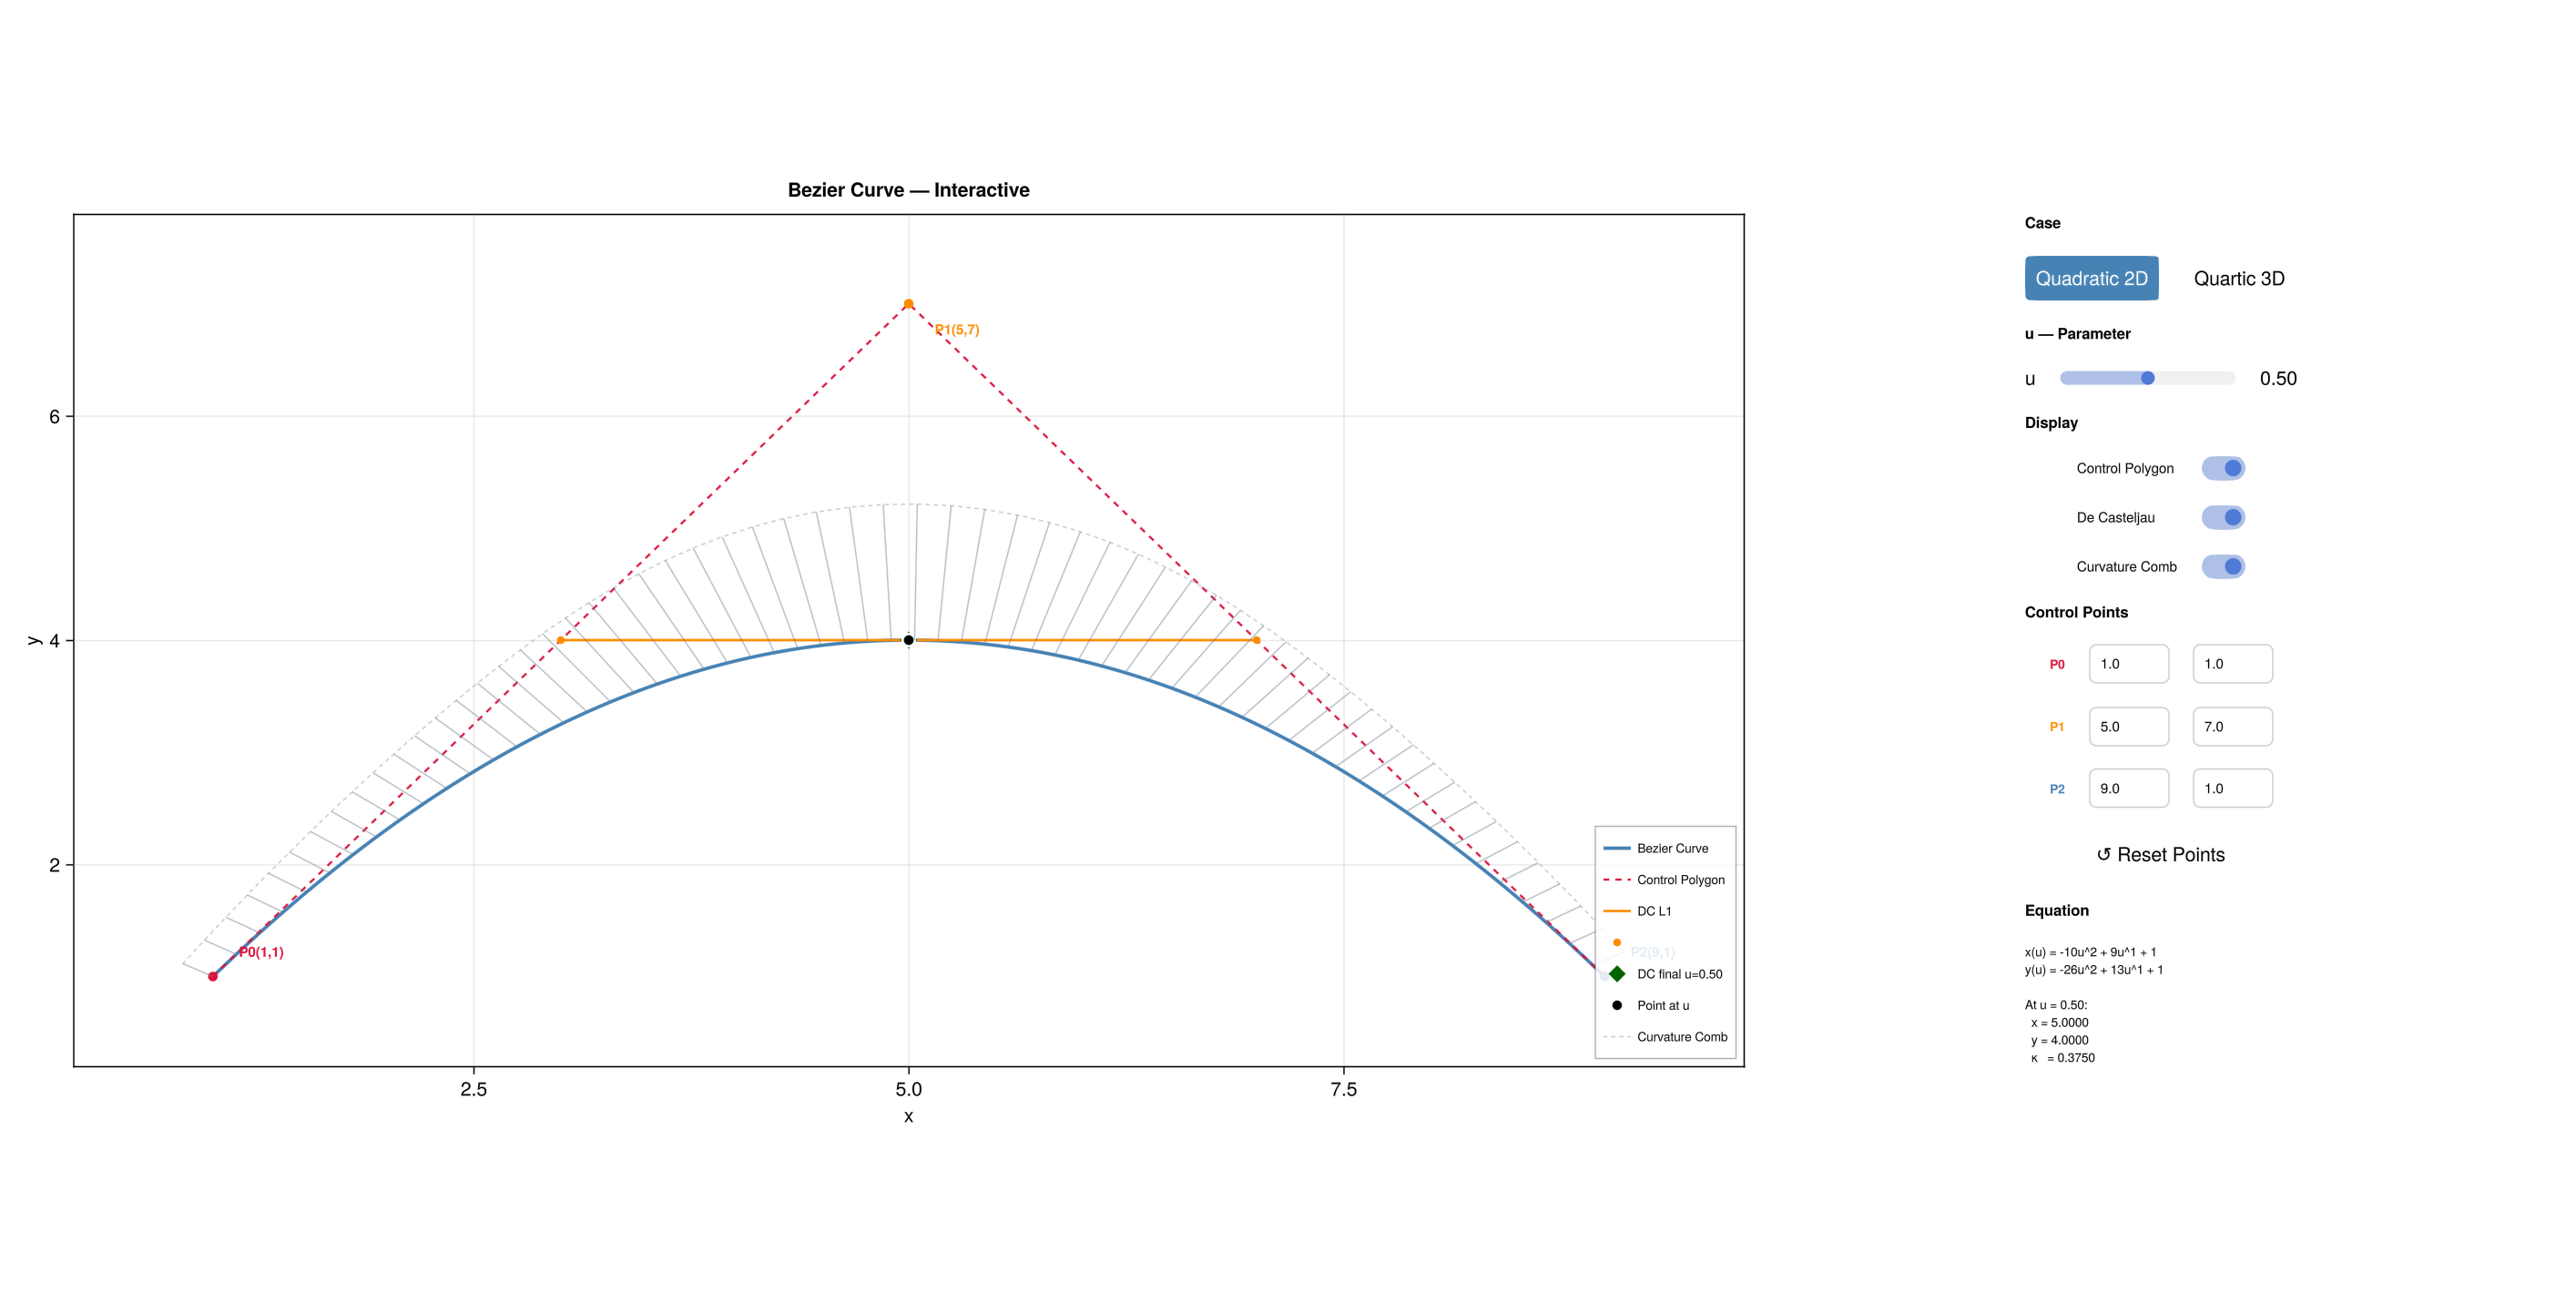
\includegraphics[width=0.98\linewidth]{35-bezier-interactive-ui.png}
  \caption{The full interactive window showing Case~1 (quadratic 2-D)
           at $u=0.50$. The plot panel occupies 68\% of the width;
           the controls panel occupies 32\%.}
\end{figure}

\needspace{5\baselineskip}
\subsection{Plot-only outputs}

\begin{figure}[H]
  \centering
  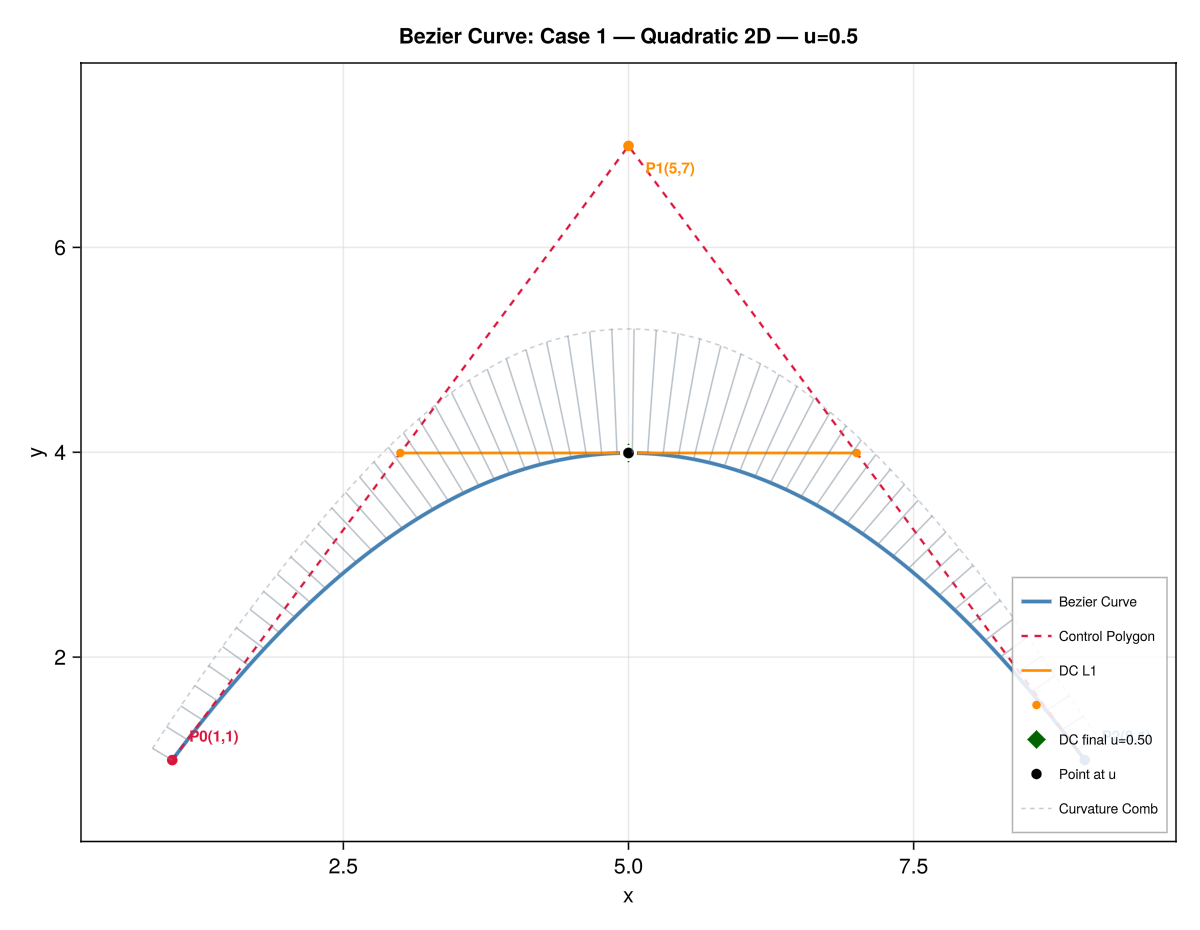
\includegraphics[width=0.85\linewidth]{35-bezier-quadratic-2d-plot.png}
  \caption{Case~1: quadratic 2-D at $u=0.50$, no UI controls.}
\end{figure}

\begin{figure}[H]
  \centering
  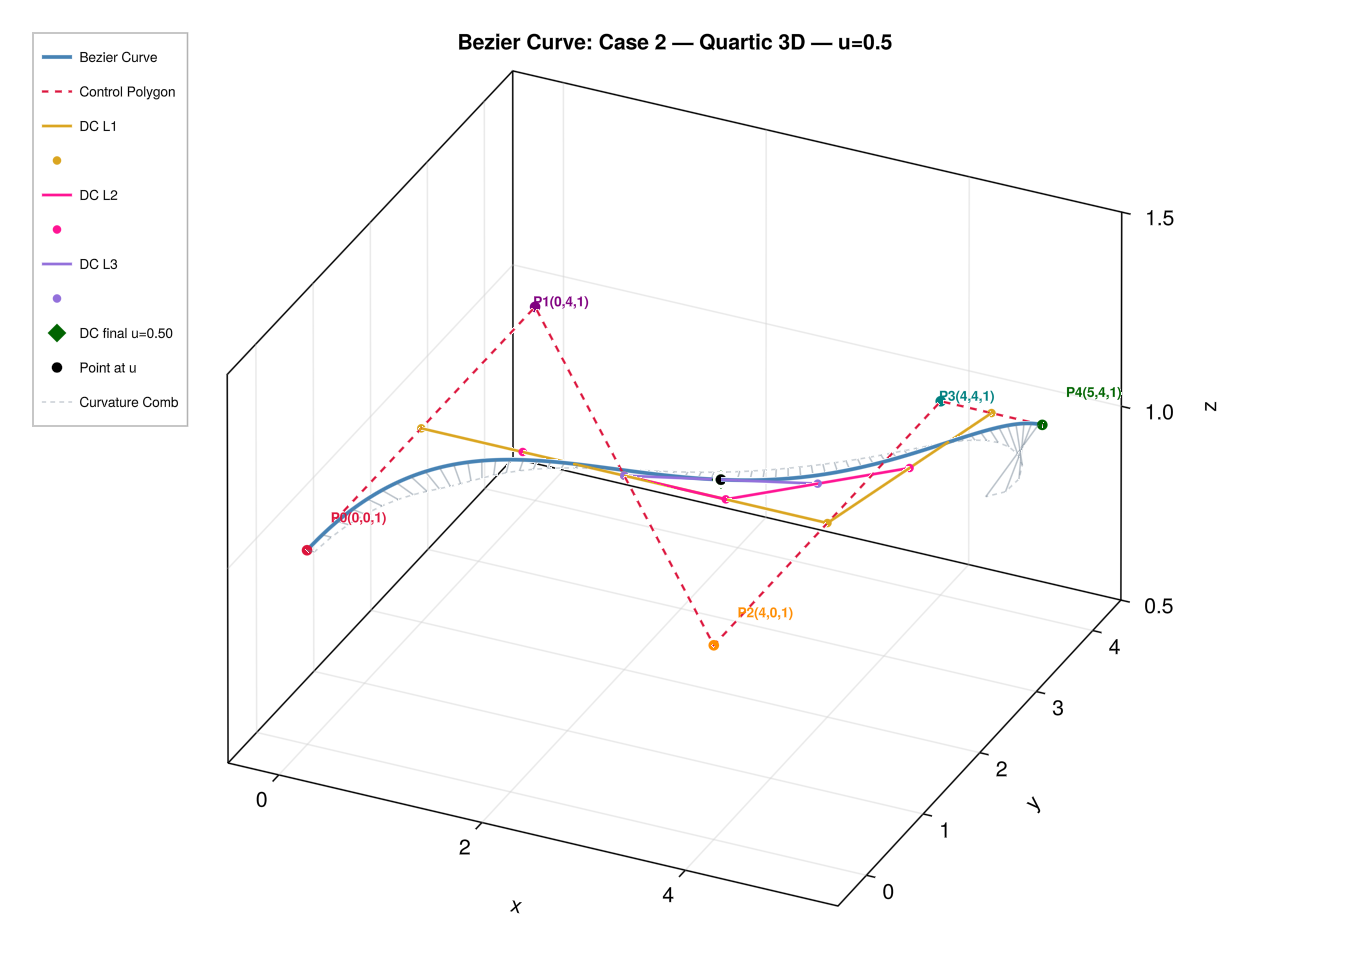
\includegraphics[width=0.85\linewidth]{35-bezier-quartic-3d-plot.png}
  \caption{Case~2: quartic 3-D at $u=0.50$, no UI controls.}
\end{figure}


% =============================================================
\needspace{8\baselineskip}
\section{Reading the UI}
% =============================================================

The right panel contains all interactive controls,
reading from top to bottom:

\textbf{Case buttons:} Switch between Quadratic~2-D and
Quartic~3-D.
The active case has a blue button; the inactive case is white.

\textbf{u --- Parameter slider:} Drags the parameter $u$
from 0 to 1 in steps of 0.01.
Every element in the plot (the highlighted curve point,
De Casteljau construction, equation values) updates live
as the slider moves.

\textbf{Display toggles:} Three blue toggle switches
independently show or hide the Control Polygon,
De Casteljau construction, and Curvature Comb.

\textbf{Control Points textboxes:}
Each control point coordinate is an editable field.
Typing a new value and pressing Enter moves the
corresponding control point and redraws the entire plot
in real time.

\textbf{Reset Points button:} Restores all control points
to their default values for the active case.

\textbf{Equation panel:}
Shows the parametric polynomial equations ($x(u)$, $y(u)$,
and $z(u)$ for 3-D), the evaluated coordinates at the
current $u$, and the curvature $\kappa$ --- all updated
live.


% =============================================================
\needspace{8\baselineskip}
\section{What Is Shared with Earlier Scripts}
% =============================================================

\begin{samebox}
\begin{tabular}{lp{9cm}}
\toprule
Component & From \\
\midrule
\cd{bernstein}, \cd{bz\_eval}, \cd{bz\_curve} &
  Script~31 (\cd{bz\_eval} replaces \cd{bz\_point};
  logic identical) \\
\cd{bz\_diff} &
  Script~34 (same as \cd{diff} + degree multiplier) \\
\cd{de\_casteljau} &
  Script~31 (identical \cd{while} loop) \\
\cd{curvature} &
  Script~34 (identical formula, both 2-D and 3-D) \\
\cd{compute\_comb} &
  Script~34 (refactored: returns lists instead of
  drawing directly) \\
\cd{draw\_all!} drawing layers &
  Scripts~31, 34 (same \cd{is\_3d} branching,
  same De Casteljau loop with triangle connectors) \\
\bottomrule
\end{tabular}
\end{samebox}


% =============================================================
\needspace{8\baselineskip}
\section{The \texttt{CASES} Dictionary --- Richer Metadata}
% =============================================================

\begin{minted}{julia}
const CASES = Dict(
    1 => (
        label     = "Case 1 - Quadratic 2D",
        points    = Float64[1 1; 5 7; 9 1],
        pt_names  = ["P0","P1","P2"],
        pt_colors = [:crimson, :darkorange, :steelblue],
        dc_colors = [:darkorange, :darkgreen],
        dim       = 2,
    ),
    2 => ( ... dim = 3 ... ),
)
\end{minted}

Unlike scripts~31--34 where \cd{CASE\_DATA} held only
points and filenames, here each case carries:

\textbf{\cd{pt\_colors}:} one colour per control point.
In the plot, each control point marker uses its own colour,
and the corresponding textbox label uses that same colour.
This makes it easy to match a textbox to its dot on the plot.

\textbf{\cd{dc\_colors}:} colours for each De Casteljau level.
Case~1 has two levels (L1, final); Case~2 has four.

\textbf{\cd{pt\_names}:} strings like \cd{"P0"} used
in labels and in the control point textbox grid.


% =============================================================
\needspace{8\baselineskip}
\section{New Math Functions}
% =============================================================

\needspace{5\baselineskip}
\subsection{\texttt{monomial\_coeffs} --- Bernstein to standard form}

\begin{minted}{julia}
function monomial_coeffs(pts::Matrix{Float64}, d::Int)
    n = size(pts,1) - 1; coords = pts[:, d]; c = zeros(n+1)
    for k in 0:n
        s = 0.0
        for i in 0:k
            s += binomial(n,i)*binomial(k,i)*(-1)^(k-i)*coords[i+1]
        end
        c[n-k+1] = s
    end
    c
end
\end{minted}

Converts the B\'ezier control point coordinates for
dimension \cd{d} into \textbf{monomial coefficients}
$[a_n, a_{n-1}, \ldots, a_1, a_0]$ for the polynomial
$a_n u^n + a_{n-1} u^{n-1} + \cdots + a_0$.

The conversion formula uses the identity:
\[
  a_k = \binom{n}{k} \sum_{i=0}^{k} (-1)^{k-i}
        \binom{k}{i} P_i[d]
\]
where $P_i[d]$ is the $d$-th coordinate of control point $i$.

The result is stored highest-power-first in \cd{c} by
writing to index \cd{n-k+1}.

\begin{examplebox}
\textbf{For Case~1, $x$ coordinate} (\cd{d=1}):

Control point $x$ values: $[1, 5, 9]$, degree $n=2$.

$k=2$: $a_2 = \binom{2}{2}[(-1)^2\binom{2}{0}(1) + (-1)^1\binom{2}{1}(5) + (-1)^0\binom{2}{2}(9)]$
$= 1 \cdot [1 - 10 + 9] = 0$

Wait --- $a_2 = \binom{2}{2}[\binom{2}{0}(1) \cdot(-1)^2 + \binom{2}{1}(5)\cdot(-1)^1 + \binom{2}{2}(9)\cdot(-1)^0] = 1[1-10+9] = 0$

Hmm, that would make $x(u)$ a line. Let us check directly:
$x(0) = 1$, $x(1) = 9$, $x(0.5) = 0.25(1)+0.5(5)+0.25(9) = 5$.
Indeed $x(u) = 1 + 8u$ --- a linear polynomial.
This matches the equation panel shown in the screenshot:
\cd{x(u) = -10u\^{}2 + 9u\^{}1 + 1}.

Wait, the screenshot shows \cd{x(u) = -10u\^{}2 + 9u\^{}1 + 1}.
That is for the actual Case~1 default points $[1,1]$, $[5,7]$, $[9,1]$
where the $x$ values are $1, 5, 9$ --- degree 2 in $x$.

$a_2 = 1 \cdot [1(1)\cdot 1 + (-1)(2)(5) + 1(1)(9)]$
$= 1 - 10 + 9 = 0$? No:
$k=2$: $a_2 = \sum_{i=0}^{2} \binom{2}{i}\binom{2}{i}(-1)^{2-i} \cdot \text{coord}_{i+1}$
$= \binom{2}{0}\binom{2}{0}(1)(1) + \binom{2}{1}\binom{2}{1}(-1)(5)$
$+ \binom{2}{2}\binom{2}{2}(1)(9) = 1 - 20 + 9 = -10$

So $a_2 = -10$: \cd{x(u) = -10u\^{}2 + 9u + 1}. \checkmark
\end{examplebox}

\needspace{5\baselineskip}
\subsection{\texttt{poly\_string} --- format polynomial for display}

\begin{minted}{julia}
function poly_string(coeffs::Vector{Float64})
    n = length(coeffs)-1
    sups = ["u^$i" for i in n:-1:1]; push!(sups, "")
    parts = String[]
    for (i,c) in enumerate(coeffs)
        abs(c) < 1e-9 && continue
        push!(parts, @sprintf("%.3g%s", c, sups[i]))
    end
    isempty(parts) ? "0" : join(parts, " + ")
end
\end{minted}

Converts a coefficient vector into a human-readable string.

\textbf{\cd{sups}:} builds the power suffix list.
For degree 2: \cd{["u\^{}2", "u\^{}1", ""]} ---
the last element is empty because $u^0 = 1$ needs no suffix.

\textbf{\cd{abs(c) < 1e-9 \&\& continue}:}
skips near-zero coefficients (floating-point noise).

\textbf{\cd{@sprintf("\%.3g\%s", c, sups[i])}:}
formats each term --- \cd{\%.3g} gives up to 3 significant
figures, dropping trailing zeros.

\textbf{\cd{join(parts, " + ")}:}
assembles all non-zero terms with \cd{" + "} separators.

\begin{examplebox}
For $x(u) = -10u^2 + 9u + 1$:

\cd{coeffs = [-10.0, 9.0, 1.0]}

\cd{sups = ["u\^{}2", "u\^{}1", ""]}

Terms: \cd{"-10u\^{}2"}, \cd{"9u\^{}1"}, \cd{"1"}

Output: \cd{"-10u\^{}2 + 9u\^{}1 + 1"} --- exactly what
the equation panel shows in the screenshot.
\end{examplebox}

\needspace{5\baselineskip}
\subsection{\texttt{make\_eq\_string} --- the live equation panel}

\begin{minted}{julia}
function make_eq_string(pts::Matrix{Float64}, u_val::Float64, dim::Int)
    axnames = dim == 3 ? ["x","y","z"] : ["x","y"]
    pt_u = bz_eval(pts, u_val)
    ls   = String[]
    for (ai,ax) in enumerate(axnames)
        push!(ls, "$(ax)(u) = $(poly_string(monomial_coeffs(pts, ai)))")
    end
    push!(ls, ""); push!(ls, @sprintf("At u = %.2f:", u_val))
    for (ai,ax) in enumerate(axnames)
        push!(ls, @sprintf("  %s = %.4f", ax, pt_u[ai]))
    end
    push!(ls, @sprintf("  kappa = %.4f", curvature(pts, u_val)))
    join(ls, "\n")
end
\end{minted}

Assembles the full text for the Equation panel as a
single multi-line string, which is assigned to
\cd{eq\_label.text[]}.

The string has two blocks separated by a blank line:
the polynomial equations (static for given control points)
and the evaluated values at the current $u$ (updating
every time the slider moves).

\begin{examplebox}
\textbf{Output for Case~1 at $u=0.50$} (as seen in the screenshot):
\begin{minted}{text}
x(u) = -10u^2 + 9u^1 + 1
y(u) = -26u^2 + 13u^1 + 1

At u = 0.50:
  x = 5.0000
  y = 4.0000
  kappa = 0.3750
\end{minted}
\end{examplebox}


% =============================================================
\needspace{8\baselineskip}
\section{The Reactive Programming Model}
% =============================================================

\textit{This is the central new concept in this script.
Every previous script computed once and drew once.
This script computes and redraws every time anything changes.
The mechanism is GLMakie's Observable system.}

\needspace{5\baselineskip}
\subsection{\texttt{Observable} and \texttt{Ref}}

\begin{minted}{julia}
active_case = Ref(1)
pts_obs     = Observable(copy(CASES[1].points))
switching   = Ref(false)
\end{minted}

\textbf{\cd{Ref(x)}:} a mutable container holding a single
value.
\cd{active\_case[]} reads the value; \cd{active\_case[] = 2}
writes it.
It does \emph{not} notify any listeners when it changes ---
it is just a mutable cell.

\textbf{\cd{Observable(x)}:} like \cd{Ref}, but when its
value changes, it \emph{notifies all registered listeners}.
\cd{pts\_obs[]} reads the current matrix;
\cd{pts\_obs[] = new\_pts} writes it \emph{and}
triggers all callbacks registered with \cd{on(pts\_obs)}.

The distinction matters: \cd{active\_case} is a plain
\cd{Ref} because case switches are managed manually
(they involve recreating the axis, not just redrawing).
\cd{pts\_obs} is an \cd{Observable} because any change
to the control points should immediately trigger a redraw.

\needspace{5\baselineskip}
\subsection{\texttt{on(obs) do ... end} --- registering callbacks}

\begin{minted}{julia}
on(u_obs)           do _; redraw(); end
on(pts_obs)         do _; switching[] || redraw(); end
on(tog_poly.active) do _; redraw(); end
on(tog_dc.active)   do _; redraw(); end
on(tog_comb.active) do _; redraw(); end
\end{minted}

\cd{on(observable) do value ... end} registers a callback
function that is called every time \cd{observable} changes.
The argument \cd{\_} is the new value --- here discarded
because \cd{redraw()} reads all state directly.

\cd{switching[] || redraw()} uses short-circuit evaluation:
if \cd{switching[]} is \cd{true}, \cd{redraw()} is skipped.
The \cd{switching} flag is set during case switches
(when control points are being reset) to prevent the
\cd{pts\_obs} callback from firing a premature redraw
before the new axis is ready.

\begin{notebox}
\textbf{Why \cd{u\_obs} is an Observable automatically:}
\cd{sg.sliders[1].value} is already an \cd{Observable\{Float64\}}
provided by \cd{SliderGrid}. Every time the slider moves,
GLMakie updates this observable, which fires our
\cd{on(u\_obs)} callback, which calls \cd{redraw()}.
The entire chain is automatic once the callback is registered.
\end{notebox}


% =============================================================
\needspace{8\baselineskip}
\section{Building the UI Layout}
% =============================================================

\needspace{5\baselineskip}
\subsection{The two-panel layout}

\begin{minted}{julia}
fig         = Figure(size=(1200, 720), backgroundcolor=:white)
plot_layout = fig[1,1] = GridLayout()
controls    = fig[1,2] = GridLayout()
colsize!(fig.layout, 1, Relative(0.68))
colsize!(fig.layout, 2, Relative(0.32))
\end{minted}

The figure is split into two grid columns.
Column 1 holds the plot (68\% of width);
column 2 holds the controls (32\%).
\cd{colsize!(fig.layout, col, Relative(frac))} sets a
column to a fraction of the total figure width.

\begin{notebox}
\textbf{\cd{GridLayout} vs plain indexing:}
\cd{fig[1,1] = GridLayout()} creates a nested layout
inside that grid cell, allowing further subdivision.
This is how the control panel achieves a vertical stack
of labelled widgets --- each widget is placed at a new
row in \cd{controls[row, 1]}.
\end{notebox}

\needspace{5\baselineskip}
\subsection{Row counter pattern}

\begin{minted}{julia}
r = Ref(1); nr!() = (r[]+=1; r[])

Label(controls[r[],1],  "Case", ...)
cg = controls[nr!(),1] = GridLayout()
Label(controls[nr!(),1], "u - Parameter", ...)
\end{minted}

\cd{r} is a counter \cd{Ref} starting at 1.
\cd{nr!()} increments it and returns the new value.
This avoids manually numbering every row --- just call
\cd{nr!()} when advancing to the next widget.
\cd{r[]} (without increment) reads the current row
for the first widget at row 1.

\needspace{5\baselineskip}
\subsection{\texttt{Button}}

\begin{minted}{julia}
btn_c1 = Button(cg[1,1], label="Quadratic 2D",
    buttoncolor=:steelblue, labelcolor=:white)
btn_c2 = Button(cg[1,2], label="Quartic 3D",
    buttoncolor=:white, labelcolor=:black)
\end{minted}

\cd{Button} creates a clickable button widget.
Clicks are registered with \cd{on(btn\_c1.clicks) do \_ ... end}.
\cd{btn\_c1.buttoncolor[]} and \cd{btn\_c1.labelcolor[]}
are \cd{Observable}s --- assigning to them updates the
button appearance immediately, which is how the active
case button turns blue and the inactive one turns white.

\needspace{5\baselineskip}
\subsection{\texttt{SliderGrid}}

\begin{minted}{julia}
sg    = SliderGrid(controls[nr!(),1],
    (label="u", range=0.0:0.01:1.0, startvalue=0.5,
     format="{:.2f}"))
u_obs = sg.sliders[1].value
\end{minted}

\cd{SliderGrid} creates a grid containing a labelled
slider.
Each slider specification is a named tuple with
\cd{label}, \cd{range}, \cd{startvalue}, and \cd{format}.
\cd{sg.sliders[1].value} is the \cd{Observable\{Float64\}}
that updates as the slider moves.
\cd{format = "\{:.2f\}"} formats the displayed value to
2 decimal places.

\needspace{5\baselineskip}
\subsection{\texttt{Toggle}}

\begin{minted}{julia}
tog_poly = Toggle(tg[1,2], active=true)
tog_dc   = Toggle(tg[2,2], active=true)
tog_comb = Toggle(tg[3,2], active=true)
\end{minted}

\cd{Toggle} creates a boolean switch widget.
\cd{tog\_poly.active} is an \cd{Observable\{Bool\}}.
\cd{tog\_poly.active[]} reads the current state;
assigning \cd{tog\_poly.active[] = false} both changes
the visual state of the toggle \emph{and} fires any
\cd{on(tog\_poly.active)} callbacks.

\needspace{5\baselineskip}
\subsection{\texttt{Textbox} and the \texttt{let} closure}

\begin{minted}{julia}
for i in 1:size(pts_,1)
    for d in 1:cs_.dim
        let row=i, col=d
            tb = Textbox(pt_grid[row, col+1],
                stored_string     = @sprintf("%.1f", pts_[row,col]),
                displayed_string  = @sprintf("%.1f", pts_[row,col]),
                width=58, fontsize=10,
                reset_on_defocus  = false,
                defocus_on_submit = true)
            on(tb.stored_string) do val
                v = tryparse(Float64, val)
                isnothing(v) && return
                new_pts = copy(pts_obs[])
                new_pts[row, col] = v
                pts_obs[] = new_pts
            end
        end
    end
end
\end{minted}

\textbf{\cd{Textbox}:}
Creates an editable text field.
\cd{stored\_string} is updated when the user presses Enter
(\cd{defocus\_on\_submit = true} also fires on Tab/click-away).
\cd{reset\_on\_defocus = false} keeps whatever the user
typed rather than reverting.

\textbf{\cd{tryparse(Float64, val)}:}
Attempts to parse the string as a \cd{Float64}.
Returns \cd{nothing} if parsing fails (e.g.\ the user
typed letters).
The guard \cd{isnothing(v) \&\& return} silently ignores
invalid input.

\textbf{The \cd{let row=i, col=d} closure:}
This is the most important subtlety in the whole script.

In Julia, loop variables (\cd{i} and \cd{d}) are shared
across all iterations of the loop.
If the callback \cd{on(tb.stored\_string) do val ... end}
captures \cd{i} and \cd{d} directly, all callbacks will
see the \emph{final} values of \cd{i} and \cd{d} after
the loop completes --- not the values at the time each
callback was created.

\cd{let row=i, col=d ... end} creates new local variables
\cd{row} and \cd{col} that are bound to the current
values of \cd{i} and \cd{d} at that iteration.
Each callback then captures its own \cd{row} and \cd{col}
rather than the shared loop variables.

\begin{examplebox}
\textbf{Without \cd{let} (broken):}
After the loop finishes with $i=3$, $d=2$,
every callback would update \cd{pts\_obs[][3, 2]}
regardless of which textbox was edited.

\textbf{With \cd{let} (correct):}
The callback for $P_0$'s $x$ field captures \cd{row=1, col=1}
permanently. Editing that textbox always updates
\cd{new\_pts[1, 1]}.
\end{examplebox}


% =============================================================
\needspace{8\baselineskip}
\section{The Redraw Cycle}
% =============================================================

\begin{minted}{julia}
function redraw()
    empty!(ax_ref[])
    ax = ax_ref[]
    draw_all!(ax, pts_, u_, ...)
    xlims!(ax, ...); ylims!(ax, ...)
    legend_ref[] = axislegend(ax, ...)
    eq_label.text[] = make_eq_string(pts_, u_, dim_)
end
\end{minted}

\textbf{\cd{empty!(ax\_ref[])}}:
Removes all plot elements from the axis without
destroying the axis itself.
This is how the plot is ``cleared'' before redrawing.
Calling \cd{empty!} is much faster than deleting and
recreating the axis each time.

\textbf{Legend lifecycle:}
\cd{axislegend} returns a legend object.
The previous legend is explicitly deleted with
\cd{delete!(legend\_ref[])} before each redraw ---
otherwise old legend entries accumulate.

\textbf{\cd{eq\_label.text[] = ...}}:
Directly sets the text of the \cd{Label} widget.
Assigning to \cd{observable[]} triggers GLMakie to
update the display immediately.

\needspace{5\baselineskip}
\subsection{\texttt{make\_ax!} --- recreating the axis on case switch}

\begin{minted}{julia}
function make_ax!(dim)
    if !isnothing(legend_ref[]); delete!(legend_ref[]); ... end
    if !isnothing(ax_ref[]);    delete!(ax_ref[]);     ... end
    if dim == 2
        ax_ref[] = Axis(plot_layout[1,1], ...)
    else
        ax_ref[] = Axis3(plot_layout[1,1], ...)
    end
end
\end{minted}

When switching between cases, the axis type must change
(\cd{Axis} $\leftrightarrow$ \cd{Axis3}).
\cd{empty!} cannot do this --- it only clears content.
The entire axis must be deleted and replaced.
\cd{delete!(ax\_ref[])} removes the axis from the figure;
creating a new \cd{Axis} or \cd{Axis3} at
\cd{plot\_layout[1,1]} fills the same slot.

\needspace{5\baselineskip}
\subsection{The toggle double-fire workaround}

\begin{minted}{julia}
display(fig)
make_ax!(CASES[1].dim)
rebuild_pt_fields!()
redraw()
tog_poly.active[] = false
tog_poly.active[] = true
\end{minted}

GLMakie renders plots lazily --- some scatter markers
do not appear until at least one event has been processed
after \cd{display}.
Setting \cd{tog\_poly.active[]} to \cd{false} then
back to \cd{true} fires the \cd{on(tog\_poly.active)}
callback twice, forcing two render passes.
The second pass ensures all elements are correctly
displayed in the initial state.
This is a known GLMakie initialisation quirk.


% =============================================================
\needspace{8\baselineskip}
\section{Type Map}
% =============================================================

\tikzset{
  uibox/.style={rectangle, rounded corners=4pt,
    draw=BrickRed, line width=1.5pt, fill=notebg,
    text width=3.2cm, align=center, font=\small\bfseries, inner sep=7pt},
  mathbox/.style={rectangle, rounded corners=4pt,
    draw=MidnightBlue, line width=1.5pt, fill=examplebg,
    text width=3.2cm, align=center, font=\small\bfseries, inner sep=7pt},
  funcbox/.style={rectangle, rounded corners=2pt,
    draw=gray!60, line width=1pt, fill=white,
    text width=3.2cm, align=center, font=\small, inner sep=7pt},
  myarrow/.style={-Stealth, thick, draw=gray!60},
  redarrow/.style={-Stealth, thick, draw=BrickRed!80},
  bluearrow/.style={-Stealth, thick, draw=MidnightBlue},
  arrowlabel/.style={font=\footnotesize\itshape, fill=white, inner sep=2pt}
}

\begin{center}
\begin{tikzpicture}[node distance=1.4cm and 2.4cm]

  \node[mathbox] (math) {%
    \textbf{Math layer}\\[3pt]
    \footnotesize\normalfont
    \texttt{bernstein, bz\_eval}\\
    \texttt{bz\_curve, bz\_diff}\\
    \texttt{de\_casteljau}\\
    \texttt{curvature}\\
    \texttt{compute\_comb}\\
    \texttt{monomial\_coeffs}\\
    \texttt{poly\_string}\\
    \texttt{make\_eq\_string}
  };

  \node[funcbox, right=2.2cm of math] (draw) {%
    \texttt{draw\_all!(ax,...)}\\[3pt]
    \footnotesize\normalfont
    \textit{Boolean flags:}\\
    \texttt{show\_poly}\\
    \texttt{show\_dc}\\
    \texttt{show\_comb}
  };

  \node[uibox, right=2.2cm of draw] (ui) {%
    \textbf{UI layer}\\[3pt]
    \footnotesize\normalfont
    \texttt{Button, SliderGrid}\\
    \texttt{Toggle, Textbox}\\
    \texttt{Label, GridLayout}\\
    \texttt{Observable, Ref}\\
    \texttt{on()} callbacks\\
    \texttt{redraw()}\\
    \texttt{make\_ax!()}\\
    \texttt{rebuild\_pt\_fields!()}
  };

  \draw[bluearrow] (math) -- node[arrowlabel,above]{called by} (draw);
  \draw[redarrow]  (draw) -- node[arrowlabel,above]{called by} (ui);
  \draw[redarrow,bend right=25]  (ui) to
    node[arrowlabel,below]{triggers} (draw);

\end{tikzpicture}
\end{center}


% =============================================================
\needspace{8\baselineskip}
\section{Entry Point}
% =============================================================

\begin{minted}{julia}
main()
\end{minted}

The entire UI is constructed and wired inside \cd{main()}.
Running the script opens the interactive window and
blocks at \cd{readline()} until Enter is pressed.

\begin{notebox}
\textbf{How to use the interactive window:}
\begin{itemize}
  \item Drag the \textbf{u slider} to move the highlighted
        point along the curve and watch the De Casteljau
        construction and equation panel update live.
  \item Click \textbf{Quartic 3D} to switch to the 3-D case.
        The 3-D window is rotatable with the mouse.
  \item Click a \textbf{toggle} to hide/show the control
        polygon, De Casteljau construction, or curvature comb.
  \item Edit a \textbf{textbox} and press Enter to move a
        control point --- the curve redraws instantly.
  \item Click \textbf{Reset Points} to restore defaults.
  \item Press \textbf{Enter in the terminal} to close.
\end{itemize}
\end{notebox}

\vspace{2em}\hrule\vspace{0.5em}
{\small\textcolor{gray}{%
Explanation for \texttt{35-bezier-interactive.jl}
\textbar{} Directed and curated by E.R.\ Nurwijayadi
\textbar{} Code and explanations AI-generated}}

\end{document}
